\begin{frame}[t]{GrPPI ideals}
\begin{itemize}[<+->]
  \item Applications should be expressed \textmark{independently} of the
        \textgood{execution model}.
  \vfill
  \item \textgood{Multiple back-ends} should be offered with \textmark{simple switching}
        mechanisms.
  \vfill
  \item Interface should \textmark{integrate} seamlessly with \textgood{modern C++} and
        its standard library.
  \vfill
  \item Applications should be able to \textmark{take advantage} of \textgood{modern C++} language features.
\end{itemize}
\end{frame}

\begin{frame}[t]{GrPPI}
\begin{Large}
\textgood{\url{https://github.com/arcosuc3m/grppi}}
\end{Large}
\vfill\pause
\begin{itemize}
  \item A header only library (might change).
  \item A set of execution policies.
  \item A set of type safe generic algorithms.
  \item Requires \textgood{C++14}.
  \item GNU GPL v3.
\end{itemize}
\end{frame}

\begin{frame}[t]{GrPPI as a teching tool}
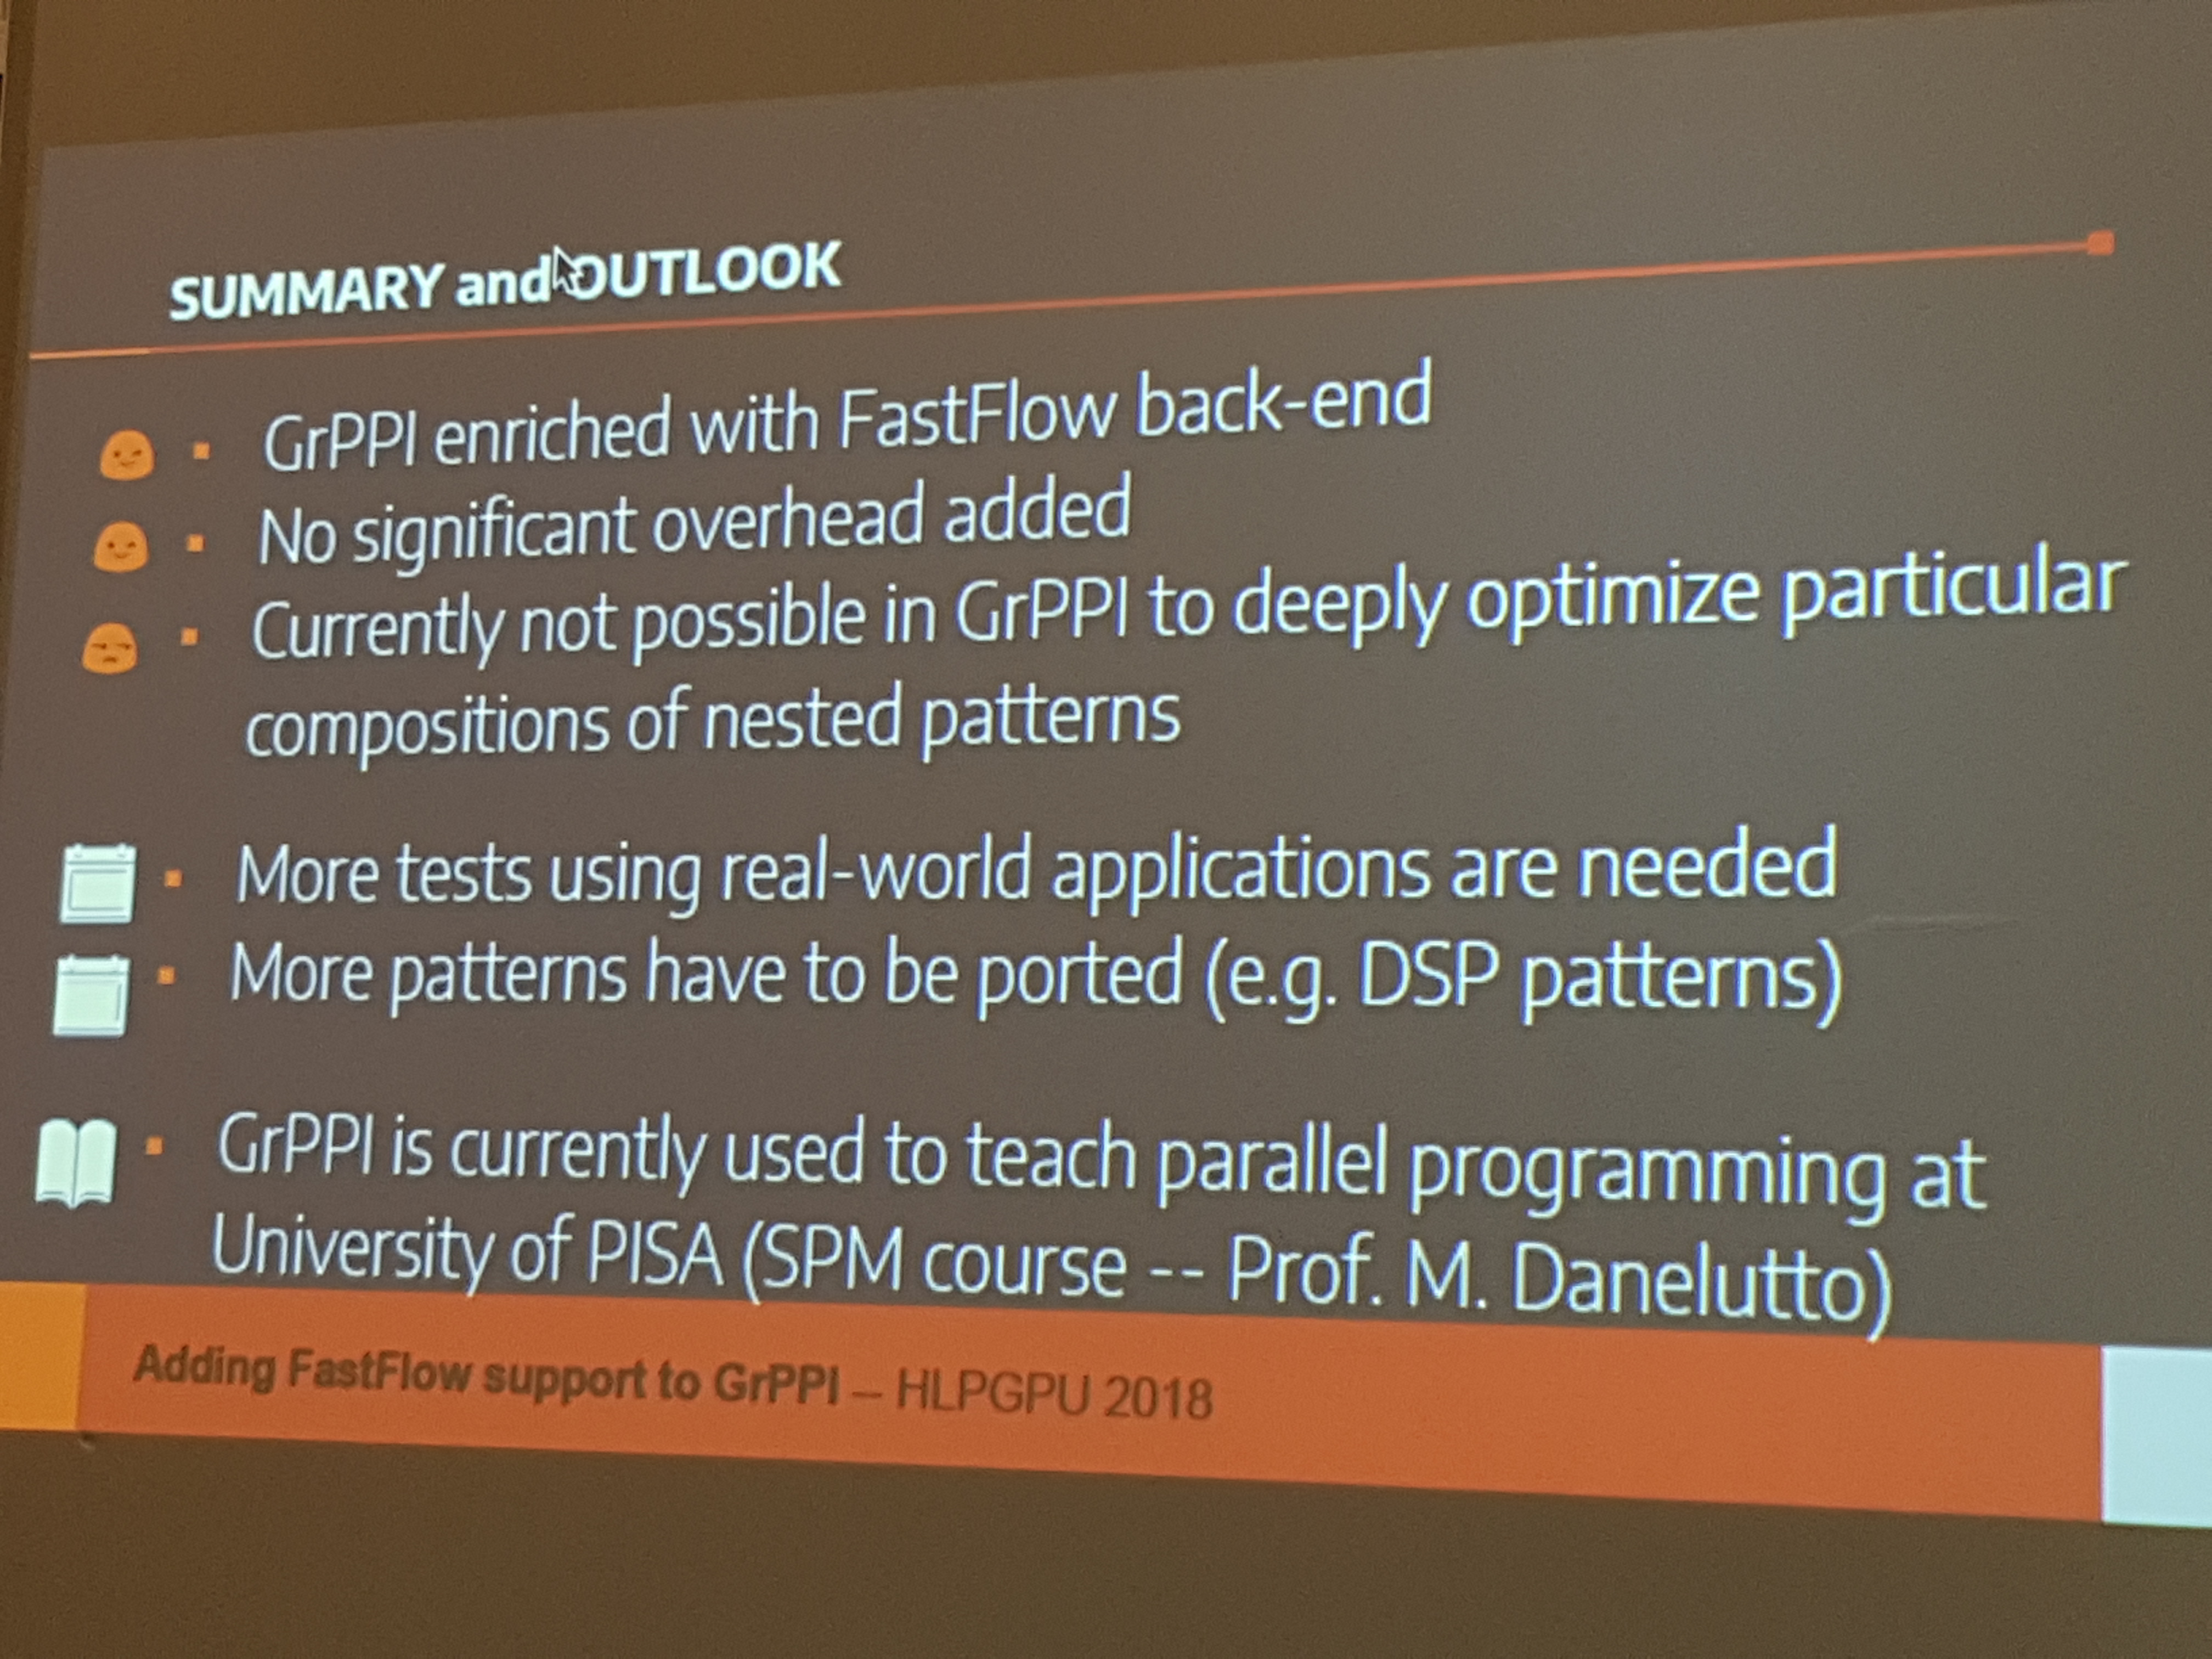
\includegraphics[width=\textwidth]{img/grppi-upi.jpg}
\end{frame}

\begin{frame}[t]{Execution policies}
\begin{itemize}
  \item The execution model is encapsulated by execution values.
    \begin{itemize}
      \item All top-level patterns take one \emph{execution} object.
    \end{itemize}
  \vfill
  \item Current execution types:
    \begin{itemize}
      \item \cppid{sequential\_execution}.
      \item \cppid{parallel\_execution\_native}.
      \item \cppid{parallel\_execution\_omp}.
      \item \cppid{parallel\_execution\_tbb}.
      \item \cppid{dynamic\_execution}.
      \item More to come soon!
    \end{itemize}
  \vfill
  \item Upcoming:
    \begin{itemize}
      \item \cppid{parallel\_execution\_ff}.
      \item \cppid{parallel\_execution\_cuda}.
    \end{itemize}
  \vfill
\end{itemize}
\end{frame}

